\documentclass{beamer}
\IfFileExists{beamerthemeUASLP1.sty}{
    \usetheme{UASLP1}
}{
    \usetheme{Madrid}
    \usecolortheme{seahorse}
}

\usepackage[utf8]{inputenc}
\usepackage[T1]{fontenc}
\usepackage{helvet}
\usepackage{listings}
\usepackage{xcolor}
\usepackage{tikz}
\usepackage{hyperref}

\lstset{
    basicstyle=\ttfamily\footnotesize,
    keywordstyle=\color{blue},
    commentstyle=\color{gray},
    stringstyle=\color{red},
    showstringspaces=false,
    breaklines=true,
    frame=single,
    numbers=left,
    numberstyle=\tiny\color{gray}
}

\title{Course 3: USP RAC Architecture}
\subtitle{Radio Access Controller \& Multiprotocol}
\author{Dr. ABDELMALEK OMAR}
\date{\today}
\institute{USP Zephyr Training Series\\Copyright \copyright{} 2025 Dr. ABDELMALEK OMAR}

\begin{document}

\begin{frame}[plain,t]
\titlepage
\end{frame}

\begin{frame}
\frametitle{Course Overview}
\framesubtitle{What You'll Learn}
\begin{itemize}
    \item Radio Access Controller (RAC)
    \begin{itemize}
        \item Priority-based scheduling
        \item Transaction management
        \item Resource arbitration
    \end{itemize}
    \item Multiprotocol Support
    \begin{itemize}
        \item Running LoRaWAN + Ranging concurrently
        \item Creating custom protocols
        \item Managing radio contention
    \end{itemize}
    \item Threading Models
    \begin{itemize}
        \item Single thread vs cooperative vs preemptive
        \item Performance and power trade-offs
    \end{itemize}
    \item Hands-On Labs (3 labs)
    \begin{itemize}
        \item Lab 3.1: Build multiprotocol sample
        \item Lab 3.2: Implement custom protocol
        \item Lab 3.3: Threading model comparison
    \end{itemize}
\end{itemize}
\end{frame}

\section{RAC Architecture}

\begin{frame}
\frametitle{What is RAC?}
\framesubtitle{Radio Access Controller}

\begin{block}{Definition}
RAC is USP's radio arbitration layer that enables multiple protocols to share a single radio transceiver without conflicts.
\end{block}

\begin{columns}[T]
\column{0.5\textwidth}
\textbf{The Problem:}
\begin{itemize}
    \item One radio, multiple protocols
    \item LoRaWAN wants to TX
    \item Ranging needs RX
    \item Who gets access?
\end{itemize}

\vspace{1em}

\textbf{Without RAC:}
\begin{itemize}
    \item Race conditions
    \item Corrupted packets
    \item Protocol conflicts
\end{itemize}

\column{0.5\textwidth}
\textbf{With RAC:}
\begin{itemize}
    \item Priority-based scheduling
    \item Fair resource allocation
    \item Preemption support
    \item Guaranteed access
\end{itemize}

\vspace{1em}

\textbf{Benefits:}
\begin{itemize}
    \item Multiple protocols coexist
    \item Deterministic behavior
    \item Easy to add protocols
    \item Production-proven
\end{itemize}
\end{columns}
\end{frame}

\begin{frame}
\frametitle{RAC Architecture}
\framesubtitle{Transaction-Based Model}

\begin{center}
\begin{tikzpicture}[scale=0.7]
    % Protocols
    \node[draw, rectangle, minimum width=2cm, minimum height=1cm, fill=blue!20] (lorawan) at (0,4) {LoRaWAN};
    \node[draw, rectangle, minimum width=2cm, minimum height=1cm, fill=green!20] (ranging) at (0,2) {Ranging};
    \node[draw, rectangle, minimum width=2cm, minimum height=1cm, fill=yellow!20] (custom) at (0,0) {Custom};

    % RAC Queue
    \node[draw, rectangle, minimum width=3cm, minimum height=4.5cm, fill=orange!10] (rac) at (5,2) {};
    \node at (5,5) {RAC Queue};

    \node[draw, rectangle, minimum width=2.5cm, minimum height=0.7cm] (t1) at (5,3.5) {TX Prio=2 (LoRaWAN)};
    \node[draw, rectangle, minimum width=2.5cm, minimum height=0.7cm] (t2) at (5,2.3) {RX Prio=1 (Ranging)};
    \node[draw, rectangle, minimum width=2.5cm, minimum height=0.7cm] (t3) at (5,1.1) {TX Prio=0 (Custom)};

    % Radio
    \node[draw, ellipse, minimum width=2cm, minimum height=1.5cm, fill=red!20] (radio) at (10,2) {Radio\\Hardware};

    % Arrows
    \draw[->, thick] (lorawan) -- (rac);
    \draw[->, thick] (ranging) -- (rac);
    \draw[->, thick] (custom) -- (rac);
    \draw[->, thick, red] (rac) -- (radio) node[midway, above] {\footnotesize Highest Priority};
\end{tikzpicture}
\end{center}

\textbf{Key Concept:} Transactions are queued by priority, highest priority executes first.
\end{frame}

\begin{frame}
\frametitle{RAC Transaction}
\framesubtitle{Lifecycle of a Radio Operation}

\begin{definition}[Transaction]
A transaction is a single radio operation (TX or RX) with associated callbacks.
\end{definition}

\textbf{Transaction Components:}
\begin{enumerate}
    \item \textbf{Priority:} 0-255 (higher = more important)
    \item \textbf{Pre-callback:} Configure radio before operation
    \item \textbf{Post-callback:} Process results after operation
    \item \textbf{Context:} User data passed to callbacks
\end{enumerate}

\vspace{1em}

\textbf{Lifecycle:}
\begin{enumerate}
    \item Protocol submits transaction via \texttt{rac\_add()}
    \item RAC queues by priority
    \item When radio available, call pre-callback
    \item Execute radio operation (TX/RX)
    \item Call post-callback with results
    \item Transaction complete
\end{enumerate}
\end{frame}

\begin{frame}[fragile]
\frametitle{Creating a Transaction}
\framesubtitle{Code Example}

\begin{lstlisting}[language=C, basicstyle=\tiny\ttfamily]
static rac_handle_t my_handle = NULL;

// Pre-callback: Configure radio for TX
static rac_status_t my_pre_callback(rac_handle_t handle, void *ctx)
{
    LOG_INF("Configuring radio for TX");

    // Set modulation parameters
    lr11xx_radio_set_lora_mod_params(...);

    // Load payload
    lr11xx_radio_write_buffer(radio, 0, payload, length);

    // Start TX
    lr11xx_radio_set_tx(radio, 0);

    return RAC_STATUS_OK;
}

// Post-callback: Check TX status
static rac_status_t my_post_callback(rac_handle_t handle, void *ctx)
{
    lr11xx_radio_irq_mask_t irq;
    lr11xx_radio_get_irq_status(radio, &irq);

    if (irq & LR11XX_RADIO_IRQ_TX_DONE) {
        LOG_INF("TX successful!");
    }

    return RAC_STATUS_FINISHED;
}
\end{lstlisting}
\end{frame}

\begin{frame}[fragile]
\frametitle{Submitting a Transaction}
\framesubtitle{Request Radio Access}

\begin{lstlisting}[language=C, basicstyle=\tiny\ttfamily]
void my_protocol_send(void)
{
    rac_params_t params = {
        .priority = 1,                    // Medium priority
        .pre_callback = my_pre_callback,
        .post_callback = my_post_callback,
        .radio_wake_up_time_ms = 10,      // Time to wake radio
        .transaction_timeout_ms = 2000,   // Max duration
        .context = NULL,                  // User data
    };

    rac_status_t status = rac_add(&params, &my_handle);

    if (status == RAC_STATUS_OK) {
        LOG_INF("Transaction queued");
    } else {
        LOG_ERR("Failed to queue: %d", status);
    }
}

// In main loop
int main(void) {
    while (1) {
        rac_run();  // Process RAC queue
        k_msleep(10);
    }
}
\end{lstlisting}
\end{frame}

\begin{frame}
\frametitle{Priority System}
\framesubtitle{Who Gets Access First?}

\begin{block}{Priority Rules}
\begin{enumerate}
    \item Higher priority = executes first
    \item Same priority = FIFO order
    \item Running transaction can be preempted by higher priority
\end{enumerate}
\end{block}

\textbf{Typical Priority Assignments:}
\begin{table}
\small
\begin{tabular}{|l|c|l|}
\hline
\textbf{Protocol} & \textbf{Priority} & \textbf{Rationale} \\
\hline
LoRaWAN (time-critical) & 3 & Must meet RX window timing \\
LoRaWAN (normal) & 2 & Important but flexible \\
Ranging & 1 & Real-time but can wait \\
Background scanning & 0 & Opportunistic \\
\hline
\end{tabular}
\end{table}

\begin{exampleblock}{Preemption Example}
If Ranging is RX (priority 1) and LoRaWAN needs TX (priority 2), RAC will:
\begin{enumerate}
    \item Stop Ranging RX
    \item Execute LoRaWAN TX
    \item Resume Ranging RX
\end{enumerate}
\end{exampleblock}
\end{frame}

\section{Multiprotocol}

\begin{frame}
\frametitle{LoRaWAN + Ranging}
\framesubtitle{Concurrent Protocol Operation}

\begin{center}
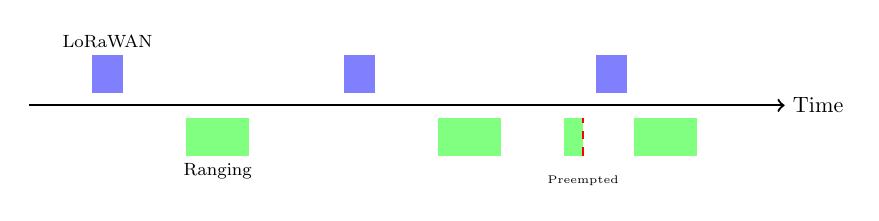
\begin{tikzpicture}[scale=0.8, transform shape]
    % Timeline
    \draw[->, thick] (0,0) -- (12,0) node[right] {Time};

    % LoRaWAN events
    \fill[blue!50] (1,0.2) rectangle (1.5,0.8) node[midway] {\tiny TX};
    \node[above] at (1.25,0.8) {\footnotesize LoRaWAN};

    \fill[blue!50] (5,0.2) rectangle (5.5,0.8) node[midway] {\tiny TX};

    \fill[blue!50] (9,0.2) rectangle (9.5,0.8) node[midway] {\tiny TX};

    % Ranging events
    \fill[green!50] (2.5,-0.8) rectangle (3.5,-0.2) node[midway] {\tiny Range};
    \node[below] at (3,-0.8) {\footnotesize Ranging};

    \fill[green!50] (6.5,-0.8) rectangle (7.5,-0.2) node[midway] {\tiny Range};

    % Preemption example
    \fill[green!50] (8.5,-0.8) rectangle (8.8,-0.2);
    \draw[red, thick, dashed] (8.8,-0.8) -- (8.8,-0.2);
    \node at (8.8,-1.2) {\tiny Preempted};
    \fill[green!50] (9.6,-0.8) rectangle (10.6,-0.2) node[midway] {\tiny Resume};
\end{tikzpicture}
\end{center}

\textbf{What Happens:}
\begin{itemize}
    \item LoRaWAN and Ranging run independently
    \item Each protocol submits transactions when needed
    \item RAC schedules based on priority
    \item LoRaWAN (higher priority) can interrupt Ranging
    \item Ranging resumes after LoRaWAN completes
\end{itemize}

\textbf{Benefits:}
\begin{itemize}
    \item Asset tracking: Position (ranging) + Cloud reporting (LoRaWAN)
    \item Smart metering: Meter reading (LoRaWAN) + Proximity detection (ranging)
\end{itemize}
\end{frame}

\begin{frame}
\frametitle{Adding Custom Protocols}
\framesubtitle{Extend USP with Your Own Protocol}

\textbf{Use Cases:}
\begin{itemize}
    \item Proprietary communication with local devices
    \item Sensor scanning in ISM bands
    \item Beacon transmission
    \item Wake-on-radio (WoR) listening
\end{itemize}

\vspace{1em}

\textbf{Requirements:}
\begin{enumerate}
    \item Implement pre-callback (configure radio)
    \item Implement post-callback (process results)
    \item Submit transactions via \texttt{rac\_add()}
    \item Choose appropriate priority (typically 0-1 for custom)
\end{enumerate}

\vspace{1em}

\textbf{Example: Heartbeat Protocol}
\begin{itemize}
    \item Broadcasts device ID every 10 seconds
    \item Uses priority 0 (lowest)
    \item Doesn't interfere with LoRaWAN
\end{itemize}
\end{frame}

\section{Threading Models}

\begin{frame}
\frametitle{Zephyr Threading Options}
\framesubtitle{How Protocols Execute}

\textbf{USP supports 3 threading models:}

\begin{enumerate}
    \item \textbf{Single Thread}
    \begin{itemize}
        \item Everything runs in \texttt{main()}
        \item Simplest, lowest memory
        \item Poor responsiveness
    \end{itemize}

    \item \textbf{Cooperative Threading}
    \begin{itemize}
        \item Protocols yield voluntarily
        \item No mutexes needed
        \item Good balance
    \end{itemize}

    \item \textbf{Preemptive Threading}
    \begin{itemize}
        \item OS preempts threads
        \item Requires mutexes for shared data
        \item Best responsiveness
        \item Highest complexity
    \end{itemize}
\end{enumerate}
\end{frame}

\begin{frame}
\frametitle{Threading Comparison}
\framesubtitle{Measured Performance}

\begin{table}
\footnotesize
\begin{tabular}{|l|c|c|c|}
\hline
\textbf{Metric} & \textbf{Single} & \textbf{Coop} & \textbf{Preempt} \\
\hline
RAM Usage & 45 KB & 48 KB & 52 KB \\
ROM Usage & 142 KB & 145 KB & 148 KB \\
Button Response & 8.5 ms & 2.3 ms & 0.85 ms \\
Avg Current (active) & 5.2 mA & 5.4 mA & 5.8 mA \\
Sleep Current & 25 µA & 28 µA & 32 µA \\
Code Complexity & Low & Medium & High \\
\hline
\end{tabular}
\end{table}

\textbf{Recommendations:}
\begin{itemize}
    \item Simple sensor: Single thread
    \item Standard IoT device: Cooperative
    \item Interactive/Real-time: Preemptive
\end{itemize}
\end{frame}

\section{Hands-On Labs}

\begin{frame}
\frametitle{Lab 3.1: Build Multiprotocol Sample}
\framesubtitle{LoRaWAN + Ranging Concurrently}

\textbf{Objective:} Run LoRaWAN and Ranging simultaneously using RAC.

\textbf{Steps:}
\begin{enumerate}
    \item Build: \texttt{west build -p -b xiao\_nrf54l15\_nrf54l15\_cpuapp \textbackslash\\
          --shield semtech\_lr1120mb1dis samples/usp/rac/multiprotocol}
    \item Configure LoRaWAN credentials
    \item Flash and monitor
    \item Use shell commands:
    \begin{itemize}
        \item \texttt{lbm join} - Join LoRaWAN network
        \item \texttt{ranging start} - Start ranging
        \item \texttt{rac status} - Check RAC queue
    \end{itemize}
\end{enumerate}

\textbf{Observations:}
\begin{itemize}
    \item LoRaWAN uplinks execute immediately (priority 2)
    \item Ranging waits if LoRaWAN is active
    \item Check RAC status to see queued transactions
\end{itemize}

\textbf{Deliverables:}
\begin{itemize}
    \item Serial log showing concurrent operation
    \item RAC status output
    \item Priority analysis document
\end{itemize}
\end{frame}

\begin{frame}[fragile]
\frametitle{Lab 3.2: Implement Custom Protocol}
\framesubtitle{Heartbeat Broadcasts}

\textbf{Objective:} Create a custom "heartbeat" protocol that coexists with LoRaWAN.

\textbf{Requirements:}
\begin{itemize}
    \item Transmit every 10 seconds
    \item Broadcast: Device ID + Uptime
    \item Priority 0 (shouldn't interfere with LoRaWAN)
    \item Frequency: 869.525 MHz (ISM band)
\end{itemize}

\textbf{Implementation Skeleton:}
\begin{lstlisting}[language=C, basicstyle=\tiny\ttfamily]
static void heartbeat_timer_handler(struct k_timer *timer)
{
    rac_params_t params = {
        .priority = 0,  // Lowest
        .pre_callback = heartbeat_pre_callback,
        .post_callback = heartbeat_post_callback,
        //...
    };
    rac_add(&params, &heartbeat_handle);
}

void heartbeat_init(void) {
    k_timer_start(&heartbeat_timer, K_SECONDS(10), K_SECONDS(10));
}
\end{lstlisting}

\textbf{Deliverables:}
\begin{itemize}
    \item Complete implementation
    \item Test showing heartbeat not blocking LoRaWAN
\end{itemize}
\end{frame}

\begin{frame}
\frametitle{Lab 3.3: Threading Model Comparison}
\framesubtitle{Measure and Compare}

\textbf{Objective:} Compare performance of single/cooperative/preemptive threading.

\textbf{Test Matrix:}
\begin{table}
\tiny
\begin{tabular}{|l|c|c|c|}
\hline
\textbf{Build Config} & \textbf{Single} & \textbf{Coop} & \textbf{Preempt} \\
\hline
CONFIG\_USP\_MAIN\_THREAD & n & y & y \\
CONFIG\_USP\_THREADS\_MUTEXES & n & n & y \\
CONFIG\_USP\_MAIN\_THREAD\_PRIORITY & - & -4 & 1 \\
\hline
\end{tabular}
\end{table}

\textbf{Measurements:}
\begin{enumerate}
    \item Build each configuration
    \item Measure RAM/ROM usage (from build output)
    \item Test button response time (microseconds)
    \item Measure power consumption (if PPK2 available)
\end{enumerate}

\textbf{Deliverables:}
\begin{itemize}
    \item Comparison table with all metrics
    \item Recommendation for specific use cases
\end{itemize}
\end{frame}

\begin{frame}
\frametitle{Course 3 Summary}
\framesubtitle{Key Takeaways}

\textbf{You've Learned:}
\begin{itemize}
    \item RAC Architecture: Priority-based radio arbitration
    \item Transactions: Pre/post callbacks for radio operations
    \item Multiprotocol: Run LoRaWAN + Ranging + Custom protocols
    \item Threading: Single vs Cooperative vs Preemptive trade-offs
    \item Practical Skills: Build multiprotocol applications, create custom protocols
\end{itemize}

\vspace{1em}

\textbf{Best Practices:}
\begin{itemize}
    \item Assign priorities carefully (time-critical = higher)
    \item Keep callbacks short and non-blocking
    \item Use cooperative threading for most applications
    \item Test multiprotocol interaction thoroughly
\end{itemize}

\vspace{1em}

\textbf{Next Course:} Course 4 - Multiprotocol Development (Ping-Pong, Ranging, PER Testing)
\end{frame}

\begin{frame}[plain]
\centering
\Huge Thank You!

\vspace{2em}

\large Questions?

\vspace{2em}

\normalsize

\end{frame}

\end{document}
